% Created by tikzDevice version 0.10.1 on 2017-12-06 18:16:12
% !TEX encoding = UTF-8 Unicode
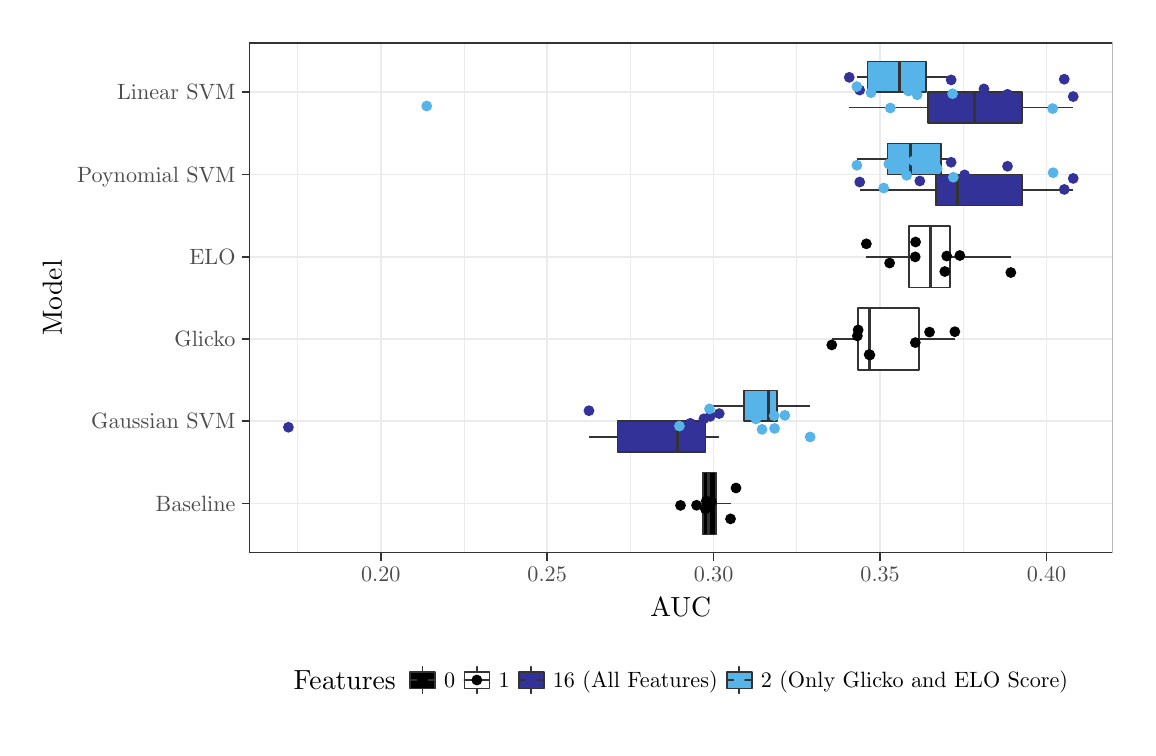
\begin{tikzpicture}[x=1pt,y=1pt]
\definecolor{fillColor}{RGB}{255,255,255}
\path[use as bounding box,fill=fillColor,fill opacity=0.00] (0,0) rectangle (397.48,252.94);
\begin{scope}
\path[clip] (  0.00,  0.00) rectangle (397.48,252.94);
\definecolor{drawColor}{RGB}{255,255,255}
\definecolor{fillColor}{RGB}{255,255,255}

\path[draw=drawColor,line width= 0.6pt,line join=round,line cap=round,fill=fillColor] (  0.00, -0.00) rectangle (397.48,252.94);
\end{scope}
\begin{scope}
\path[clip] ( 80.05, 63.15) rectangle (391.98,247.44);
\definecolor{fillColor}{RGB}{255,255,255}

\path[fill=fillColor] ( 80.05, 63.15) rectangle (391.98,247.45);
\definecolor{drawColor}{gray}{0.92}

\path[draw=drawColor,line width= 0.3pt,line join=round] ( 97.50, 63.15) --
	( 97.50,247.44);

\path[draw=drawColor,line width= 0.3pt,line join=round] (157.65, 63.15) --
	(157.65,247.44);

\path[draw=drawColor,line width= 0.3pt,line join=round] (217.80, 63.15) --
	(217.80,247.44);

\path[draw=drawColor,line width= 0.3pt,line join=round] (277.95, 63.15) --
	(277.95,247.44);

\path[draw=drawColor,line width= 0.3pt,line join=round] (338.11, 63.15) --
	(338.11,247.44);

\path[draw=drawColor,line width= 0.6pt,line join=round] ( 80.05, 80.99) --
	(391.98, 80.99);

\path[draw=drawColor,line width= 0.6pt,line join=round] ( 80.05,110.71) --
	(391.98,110.71);

\path[draw=drawColor,line width= 0.6pt,line join=round] ( 80.05,140.44) --
	(391.98,140.44);

\path[draw=drawColor,line width= 0.6pt,line join=round] ( 80.05,170.16) --
	(391.98,170.16);

\path[draw=drawColor,line width= 0.6pt,line join=round] ( 80.05,199.89) --
	(391.98,199.89);

\path[draw=drawColor,line width= 0.6pt,line join=round] ( 80.05,229.61) --
	(391.98,229.61);

\path[draw=drawColor,line width= 0.6pt,line join=round] (127.57, 63.15) --
	(127.57,247.44);

\path[draw=drawColor,line width= 0.6pt,line join=round] (187.72, 63.15) --
	(187.72,247.44);

\path[draw=drawColor,line width= 0.6pt,line join=round] (247.88, 63.15) --
	(247.88,247.44);

\path[draw=drawColor,line width= 0.6pt,line join=round] (308.03, 63.15) --
	(308.03,247.44);

\path[draw=drawColor,line width= 0.6pt,line join=round] (368.18, 63.15) --
	(368.18,247.44);
\definecolor{drawColor}{gray}{0.20}

\path[draw=drawColor,line width= 0.6pt,line join=round] (248.80, 80.99) -- (253.97, 80.99);

\path[draw=drawColor,line width= 0.6pt,line join=round] (244.08, 80.99) -- (241.71, 80.99);
\definecolor{fillColor}{RGB}{0,0,0}

\path[draw=drawColor,line width= 0.6pt,line join=round,line cap=round,fill=fillColor] (248.80, 69.84) --
	(244.08, 69.84) --
	(244.08, 92.14) --
	(248.80, 92.14) --
	(248.80, 69.84) --
	cycle;

\path[draw=drawColor,line width= 1.1pt,line join=round] (246.01, 69.84) -- (246.01, 92.14);

\path[draw=drawColor,line width= 0.6pt,line join=round] (244.91,105.14) -- (249.89,105.14);

\path[draw=drawColor,line width= 0.6pt,line join=round] (213.18,105.14) -- (202.83,105.14);
\definecolor{fillColor}{RGB}{50,50,153}

\path[draw=drawColor,line width= 0.6pt,line join=round,line cap=round,fill=fillColor] (244.91, 99.57) --
	(213.18, 99.57) --
	(213.18,110.71) --
	(244.91,110.71) --
	(244.91, 99.57) --
	cycle;

\path[draw=drawColor,line width= 1.1pt,line join=round] (234.73, 99.57) -- (234.73,110.71);

\path[draw=drawColor,line width= 0.6pt,line join=round] (270.81,116.29) -- (282.73,116.29);

\path[draw=drawColor,line width= 0.6pt,line join=round] (258.96,116.29) -- (246.37,116.29);
\definecolor{fillColor}{RGB}{86,180,233}

\path[draw=drawColor,line width= 0.6pt,line join=round,line cap=round,fill=fillColor] (270.81,110.71) --
	(258.96,110.71) --
	(258.96,121.86) --
	(270.81,121.86) --
	(270.81,110.71) --
	cycle;

\path[draw=drawColor,line width= 1.1pt,line join=round] (267.56,110.71) -- (267.56,121.86);

\path[draw=drawColor,line width= 0.6pt,line join=round] (322.04,140.44) -- (335.05,140.44);

\path[draw=drawColor,line width= 0.6pt,line join=round] (300.03,140.44) -- (290.57,140.44);
\definecolor{fillColor}{RGB}{255,255,255}

\path[draw=drawColor,line width= 0.6pt,line join=round,line cap=round,fill=fillColor] (322.04,129.29) --
	(300.03,129.29) --
	(300.03,151.58) --
	(322.04,151.58) --
	(322.04,129.29) --
	cycle;

\path[draw=drawColor,line width= 1.1pt,line join=round] (304.20,129.29) -- (304.20,151.58);

\path[draw=drawColor,line width= 0.6pt,line join=round] (333.27,170.16) -- (355.24,170.16);

\path[draw=drawColor,line width= 0.6pt,line join=round] (318.39,170.16) -- (303.06,170.16);

\path[draw=drawColor,line width= 0.6pt,line join=round,line cap=round,fill=fillColor] (333.27,159.02) --
	(318.39,159.02) --
	(318.39,181.31) --
	(333.27,181.31) --
	(333.27,159.02) --
	cycle;

\path[draw=drawColor,line width= 1.1pt,line join=round] (326.14,159.02) -- (326.14,181.31);

\path[draw=drawColor,line width= 0.6pt,line join=round] (359.18,194.31) -- (377.80,194.31);

\path[draw=drawColor,line width= 0.6pt,line join=round] (328.30,194.31) -- (300.65,194.31);
\definecolor{fillColor}{RGB}{50,50,153}

\path[draw=drawColor,line width= 0.6pt,line join=round,line cap=round,fill=fillColor] (359.18,188.74) --
	(328.30,188.74) --
	(328.30,199.89) --
	(359.18,199.89) --
	(359.18,188.74) --
	cycle;

\path[draw=drawColor,line width= 1.1pt,line join=round] (336.11,188.74) -- (336.11,199.89);

\path[draw=drawColor,line width= 0.6pt,line join=round] (330.11,205.46) -- (334.49,205.46);

\path[draw=drawColor,line width= 0.6pt,line join=round] (310.69,205.46) -- (299.62,205.46);
\definecolor{fillColor}{RGB}{86,180,233}

\path[draw=drawColor,line width= 0.6pt,line join=round,line cap=round,fill=fillColor] (330.11,199.89) --
	(310.69,199.89) --
	(310.69,211.03) --
	(330.11,211.03) --
	(330.11,199.89) --
	cycle;

\path[draw=drawColor,line width= 1.1pt,line join=round] (318.88,199.89) -- (318.88,211.03);

\path[draw=drawColor,line width= 0.6pt,line join=round] (359.18,224.04) -- (377.80,224.04);

\path[draw=drawColor,line width= 0.6pt,line join=round] (325.43,224.04) -- (296.89,224.04);
\definecolor{fillColor}{RGB}{50,50,153}

\path[draw=drawColor,line width= 0.6pt,line join=round,line cap=round,fill=fillColor] (359.18,218.46) --
	(325.43,218.46) --
	(325.43,229.61) --
	(359.18,229.61) --
	(359.18,218.46) --
	cycle;

\path[draw=drawColor,line width= 1.1pt,line join=round] (342.03,218.46) -- (342.03,229.61);

\path[draw=drawColor,line width= 0.6pt,line join=round] (324.63,235.18) -- (334.21,235.18);

\path[draw=drawColor,line width= 0.6pt,line join=round] (303.47,235.18) -- (299.62,235.18);
\definecolor{fillColor}{RGB}{86,180,233}

\path[draw=drawColor,line width= 0.6pt,line join=round,line cap=round,fill=fillColor] (324.63,229.61) --
	(303.47,229.61) --
	(303.47,240.76) --
	(324.63,240.76) --
	(324.63,229.61) --
	cycle;

\path[draw=drawColor,line width= 1.1pt,line join=round] (315.00,229.61) -- (315.00,240.76);
\definecolor{fillColor}{RGB}{0,0,0}

\path[fill=fillColor] (235.90, 80.31) circle (  1.96);

\path[fill=fillColor] (246.79, 81.46) circle (  1.96);

\path[fill=fillColor] (241.70, 80.36) circle (  1.96);

\path[fill=fillColor] (247.07, 81.61) circle (  1.96);

\path[fill=fillColor] (244.88, 79.06) circle (  1.96);

\path[fill=fillColor] (255.96, 86.60) circle (  1.96);

\path[fill=fillColor] (253.97, 75.44) circle (  1.96);

\path[fill=fillColor] (245.22, 81.94) circle (  1.96);

\path[fill=fillColor] (311.46,167.89) circle (  1.96);

\path[fill=fillColor] (332.09,170.42) circle (  1.96);

\path[fill=fillColor] (303.05,174.82) circle (  1.96);

\path[fill=fillColor] (320.85,175.49) circle (  1.96);

\path[fill=fillColor] (336.83,170.61) circle (  1.96);

\path[fill=fillColor] (331.41,164.82) circle (  1.96);

\path[fill=fillColor] (320.71,170.11) circle (  1.96);

\path[fill=fillColor] (355.26,164.46) circle (  1.96);
\definecolor{fillColor}{RGB}{50,50,153}

\path[fill=fillColor] (244.35,111.61) circle (  1.96);

\path[fill=fillColor] (246.62,112.48) circle (  1.96);

\path[fill=fillColor] (239.44,109.97) circle (  1.96);

\path[fill=fillColor] (202.82,114.53) circle (  1.96);

\path[fill=fillColor] (216.62,104.98) circle (  1.96);

\path[fill=fillColor] (249.90,113.49) circle (  1.96);

\path[fill=fillColor] (230.03,107.72) circle (  1.96);

\path[fill=fillColor] ( 94.22,108.55) circle (  1.96);
\definecolor{fillColor}{RGB}{86,180,233}

\path[fill=fillColor] (273.60,112.84) circle (  1.96);

\path[fill=fillColor] (282.74,105.05) circle (  1.96);

\path[fill=fillColor] (263.14,111.55) circle (  1.96);

\path[fill=fillColor] (265.36,107.79) circle (  1.96);

\path[fill=fillColor] (235.51,108.98) circle (  1.96);

\path[fill=fillColor] (269.89,108.12) circle (  1.96);

\path[fill=fillColor] (269.76,112.72) circle (  1.96);

\path[fill=fillColor] (246.37,115.18) circle (  1.96);
\definecolor{fillColor}{RGB}{0,0,0}

\path[fill=fillColor] (300.09,143.71) circle (  1.96);

\path[fill=fillColor] (304.07,134.81) circle (  1.96);

\path[fill=fillColor] (290.56,138.30) circle (  1.96);

\path[fill=fillColor] (335.04,143.08) circle (  1.96);

\path[fill=fillColor] (325.89,142.94) circle (  1.96);

\path[fill=fillColor] (299.81,141.56) circle (  1.96);

\path[fill=fillColor] (320.75,139.13) circle (  1.96);

\path[fill=fillColor] (304.33,134.66) circle (  1.96);
\definecolor{fillColor}{RGB}{50,50,153}

\path[fill=fillColor] (354.06,228.85) circle (  1.96);

\path[fill=fillColor] (296.88,234.99) circle (  1.96);

\path[fill=fillColor] (333.70,234.06) circle (  1.96);

\path[fill=fillColor] (300.65,230.39) circle (  1.96);

\path[fill=fillColor] (338.53,226.75) circle (  1.96);

\path[fill=fillColor] (345.54,230.81) circle (  1.96);

\path[fill=fillColor] (374.56,234.31) circle (  1.96);

\path[fill=fillColor] (377.81,228.04) circle (  1.96);
\definecolor{fillColor}{RGB}{86,180,233}

\path[fill=fillColor] (311.72,223.91) circle (  1.96);

\path[fill=fillColor] (334.21,229.07) circle (  1.96);

\path[fill=fillColor] (318.28,230.04) circle (  1.96);

\path[fill=fillColor] (144.20,224.63) circle (  1.96);

\path[fill=fillColor] (299.61,231.64) circle (  1.96);

\path[fill=fillColor] (304.74,229.46) circle (  1.96);

\path[fill=fillColor] (321.42,228.69) circle (  1.96);

\path[fill=fillColor] (370.37,223.70) circle (  1.96);
\definecolor{fillColor}{RGB}{50,50,153}

\path[fill=fillColor] (338.55,199.73) circle (  1.96);

\path[fill=fillColor] (300.66,197.16) circle (  1.96);

\path[fill=fillColor] (354.06,202.86) circle (  1.96);

\path[fill=fillColor] (333.69,204.30) circle (  1.96);

\path[fill=fillColor] (330.27,197.54) circle (  1.96);

\path[fill=fillColor] (377.81,198.47) circle (  1.96);

\path[fill=fillColor] (322.37,197.54) circle (  1.96);

\path[fill=fillColor] (374.58,194.48) circle (  1.96);
\definecolor{fillColor}{RGB}{86,180,233}

\path[fill=fillColor] (317.62,199.59) circle (  1.96);

\path[fill=fillColor] (311.16,203.71) circle (  1.96);

\path[fill=fillColor] (334.49,198.89) circle (  1.96);

\path[fill=fillColor] (370.55,200.53) circle (  1.96);

\path[fill=fillColor] (320.15,204.82) circle (  1.96);

\path[fill=fillColor] (299.63,203.23) circle (  1.96);

\path[fill=fillColor] (328.65,202.01) circle (  1.96);

\path[fill=fillColor] (309.32,195.00) circle (  1.96);

\path[draw=drawColor,line width= 0.6pt,line join=round,line cap=round] ( 80.05, 63.15) rectangle (391.98,247.45);
\end{scope}
\begin{scope}
\path[clip] (  0.00,  0.00) rectangle (397.48,252.94);
\definecolor{drawColor}{gray}{0.30}

\node[text=drawColor,anchor=base east,inner sep=0pt, outer sep=0pt, scale=  0.80] at ( 75.10, 78.23) {Baseline};

\node[text=drawColor,anchor=base east,inner sep=0pt, outer sep=0pt, scale=  0.80] at ( 75.10,107.96) {Gaussian SVM};

\node[text=drawColor,anchor=base east,inner sep=0pt, outer sep=0pt, scale=  0.80] at ( 75.10,137.68) {Glicko};

\node[text=drawColor,anchor=base east,inner sep=0pt, outer sep=0pt, scale=  0.80] at ( 75.10,167.41) {ELO};

\node[text=drawColor,anchor=base east,inner sep=0pt, outer sep=0pt, scale=  0.80] at ( 75.10,197.13) {Poynomial SVM};

\node[text=drawColor,anchor=base east,inner sep=0pt, outer sep=0pt, scale=  0.80] at ( 75.10,226.86) {Linear SVM};
\end{scope}
\begin{scope}
\path[clip] (  0.00,  0.00) rectangle (397.48,252.94);
\definecolor{drawColor}{gray}{0.20}

\path[draw=drawColor,line width= 0.6pt,line join=round] ( 77.30, 80.99) --
	( 80.05, 80.99);

\path[draw=drawColor,line width= 0.6pt,line join=round] ( 77.30,110.71) --
	( 80.05,110.71);

\path[draw=drawColor,line width= 0.6pt,line join=round] ( 77.30,140.44) --
	( 80.05,140.44);

\path[draw=drawColor,line width= 0.6pt,line join=round] ( 77.30,170.16) --
	( 80.05,170.16);

\path[draw=drawColor,line width= 0.6pt,line join=round] ( 77.30,199.89) --
	( 80.05,199.89);

\path[draw=drawColor,line width= 0.6pt,line join=round] ( 77.30,229.61) --
	( 80.05,229.61);
\end{scope}
\begin{scope}
\path[clip] (  0.00,  0.00) rectangle (397.48,252.94);
\definecolor{drawColor}{gray}{0.20}

\path[draw=drawColor,line width= 0.6pt,line join=round] (127.57, 60.40) --
	(127.57, 63.15);

\path[draw=drawColor,line width= 0.6pt,line join=round] (187.72, 60.40) --
	(187.72, 63.15);

\path[draw=drawColor,line width= 0.6pt,line join=round] (247.88, 60.40) --
	(247.88, 63.15);

\path[draw=drawColor,line width= 0.6pt,line join=round] (308.03, 60.40) --
	(308.03, 63.15);

\path[draw=drawColor,line width= 0.6pt,line join=round] (368.18, 60.40) --
	(368.18, 63.15);
\end{scope}
\begin{scope}
\path[clip] (  0.00,  0.00) rectangle (397.48,252.94);
\definecolor{drawColor}{gray}{0.30}

\node[text=drawColor,anchor=base,inner sep=0pt, outer sep=0pt, scale=  0.80] at (127.57, 52.69) {0.20};

\node[text=drawColor,anchor=base,inner sep=0pt, outer sep=0pt, scale=  0.80] at (187.72, 52.69) {0.25};

\node[text=drawColor,anchor=base,inner sep=0pt, outer sep=0pt, scale=  0.80] at (247.88, 52.69) {0.30};

\node[text=drawColor,anchor=base,inner sep=0pt, outer sep=0pt, scale=  0.80] at (308.03, 52.69) {0.35};

\node[text=drawColor,anchor=base,inner sep=0pt, outer sep=0pt, scale=  0.80] at (368.18, 52.69) {0.40};
\end{scope}
\begin{scope}
\path[clip] (  0.00,  0.00) rectangle (397.48,252.94);
\definecolor{drawColor}{RGB}{0,0,0}

\node[text=drawColor,anchor=base,inner sep=0pt, outer sep=0pt, scale=  1.00] at (236.02, 40.31) {AUC};
\end{scope}
\begin{scope}
\path[clip] (  0.00,  0.00) rectangle (397.48,252.94);
\definecolor{drawColor}{RGB}{0,0,0}

\node[text=drawColor,rotate= 90.00,anchor=base,inner sep=0pt, outer sep=0pt, scale=  1.00] at ( 12.39,155.30) {Model};
\end{scope}
\begin{scope}
\path[clip] (  0.00,  0.00) rectangle (397.48,252.94);
\definecolor{fillColor}{RGB}{255,255,255}

\path[fill=fillColor] ( 90.45,  5.50) rectangle (381.58, 28.93);
\end{scope}
\begin{scope}
\path[clip] (  0.00,  0.00) rectangle (397.48,252.94);
\definecolor{drawColor}{RGB}{0,0,0}

\node[text=drawColor,anchor=base west,inner sep=0pt, outer sep=0pt, scale=  1.00] at ( 96.14, 13.77) {Features};
\end{scope}
\begin{scope}
\path[clip] (  0.00,  0.00) rectangle (397.48,252.94);
\definecolor{fillColor}{RGB}{255,255,255}

\path[fill=fillColor] (136.63, 11.19) rectangle (148.68, 23.24);
\end{scope}
\begin{scope}
\path[clip] (  0.00,  0.00) rectangle (397.48,252.94);
\definecolor{drawColor}{gray}{0.20}

\path[draw=drawColor,line width= 0.6pt,line join=round,line cap=round] (142.65, 12.40) --
	(142.65, 14.20);

\path[draw=drawColor,line width= 0.6pt,line join=round,line cap=round] (142.65, 20.22) --
	(142.65, 22.03);
\definecolor{fillColor}{RGB}{0,0,0}

\path[draw=drawColor,line width= 0.6pt,line join=round,line cap=round,fill=fillColor] (138.14, 14.20) rectangle (147.17, 20.22);

\path[draw=drawColor,line width= 0.6pt,line join=round,line cap=round] (138.14, 17.21) --
	(147.17, 17.21);
\end{scope}
\begin{scope}
\path[clip] (  0.00,  0.00) rectangle (397.48,252.94);
\definecolor{fillColor}{RGB}{0,0,0}

\path[fill=fillColor] (142.65, 17.21) circle (  1.96);
\end{scope}
\begin{scope}
\path[clip] (  0.00,  0.00) rectangle (397.48,252.94);
\definecolor{fillColor}{RGB}{255,255,255}

\path[fill=fillColor] (156.29, 11.19) rectangle (168.33, 23.24);
\end{scope}
\begin{scope}
\path[clip] (  0.00,  0.00) rectangle (397.48,252.94);
\definecolor{drawColor}{gray}{0.20}

\path[draw=drawColor,line width= 0.6pt,line join=round,line cap=round] (162.31, 12.40) --
	(162.31, 14.20);

\path[draw=drawColor,line width= 0.6pt,line join=round,line cap=round] (162.31, 20.22) --
	(162.31, 22.03);
\definecolor{fillColor}{RGB}{255,255,255}

\path[draw=drawColor,line width= 0.6pt,line join=round,line cap=round,fill=fillColor] (157.79, 14.20) rectangle (166.83, 20.22);

\path[draw=drawColor,line width= 0.6pt,line join=round,line cap=round] (157.79, 17.21) --
	(166.83, 17.21);
\end{scope}
\begin{scope}
\path[clip] (  0.00,  0.00) rectangle (397.48,252.94);
\definecolor{fillColor}{RGB}{0,0,0}

\path[fill=fillColor] (162.31, 17.21) circle (  1.96);
\end{scope}
\begin{scope}
\path[clip] (  0.00,  0.00) rectangle (397.48,252.94);
\definecolor{fillColor}{RGB}{255,255,255}

\path[fill=fillColor] (175.95, 11.19) rectangle (187.99, 23.24);
\end{scope}
\begin{scope}
\path[clip] (  0.00,  0.00) rectangle (397.48,252.94);
\definecolor{drawColor}{gray}{0.20}

\path[draw=drawColor,line width= 0.6pt,line join=round,line cap=round] (181.97, 12.40) --
	(181.97, 14.20);

\path[draw=drawColor,line width= 0.6pt,line join=round,line cap=round] (181.97, 20.22) --
	(181.97, 22.03);
\definecolor{fillColor}{RGB}{50,50,153}

\path[draw=drawColor,line width= 0.6pt,line join=round,line cap=round,fill=fillColor] (177.45, 14.20) rectangle (186.49, 20.22);

\path[draw=drawColor,line width= 0.6pt,line join=round,line cap=round] (177.45, 17.21) --
	(186.49, 17.21);
\end{scope}
\begin{scope}
\path[clip] (  0.00,  0.00) rectangle (397.48,252.94);
\definecolor{fillColor}{RGB}{50,50,153}

\path[fill=fillColor] (181.97, 17.21) circle (  1.96);
\end{scope}
\begin{scope}
\path[clip] (  0.00,  0.00) rectangle (397.48,252.94);
\definecolor{fillColor}{RGB}{255,255,255}

\path[fill=fillColor] (251.10, 11.19) rectangle (263.15, 23.24);
\end{scope}
\begin{scope}
\path[clip] (  0.00,  0.00) rectangle (397.48,252.94);
\definecolor{drawColor}{gray}{0.20}

\path[draw=drawColor,line width= 0.6pt,line join=round,line cap=round] (257.12, 12.40) --
	(257.12, 14.20);

\path[draw=drawColor,line width= 0.6pt,line join=round,line cap=round] (257.12, 20.22) --
	(257.12, 22.03);
\definecolor{fillColor}{RGB}{86,180,233}

\path[draw=drawColor,line width= 0.6pt,line join=round,line cap=round,fill=fillColor] (252.61, 14.20) rectangle (261.64, 20.22);

\path[draw=drawColor,line width= 0.6pt,line join=round,line cap=round] (252.61, 17.21) --
	(261.64, 17.21);
\end{scope}
\begin{scope}
\path[clip] (  0.00,  0.00) rectangle (397.48,252.94);
\definecolor{fillColor}{RGB}{86,180,233}

\path[fill=fillColor] (257.12, 17.21) circle (  1.96);
\end{scope}
\begin{scope}
\path[clip] (  0.00,  0.00) rectangle (397.48,252.94);
\definecolor{drawColor}{RGB}{0,0,0}

\node[text=drawColor,anchor=base west,inner sep=0pt, outer sep=0pt, scale=  0.80] at (150.48, 14.46) {0};
\end{scope}
\begin{scope}
\path[clip] (  0.00,  0.00) rectangle (397.48,252.94);
\definecolor{drawColor}{RGB}{0,0,0}

\node[text=drawColor,anchor=base west,inner sep=0pt, outer sep=0pt, scale=  0.80] at (170.14, 14.46) {1};
\end{scope}
\begin{scope}
\path[clip] (  0.00,  0.00) rectangle (397.48,252.94);
\definecolor{drawColor}{RGB}{0,0,0}

\node[text=drawColor,anchor=base west,inner sep=0pt, outer sep=0pt, scale=  0.80] at (189.80, 14.46) {16 (All Features)};
\end{scope}
\begin{scope}
\path[clip] (  0.00,  0.00) rectangle (397.48,252.94);
\definecolor{drawColor}{RGB}{0,0,0}

\node[text=drawColor,anchor=base west,inner sep=0pt, outer sep=0pt, scale=  0.80] at (264.95, 14.46) {2 (Only Glicko and ELO Score)};
\end{scope}
\end{tikzpicture}
